\chapter{Physical System}
We consider a two-dimensional SNS-junction in the $xy$-plane and parallel to the $x$-axis, with $x=-L/2$ and $x=L/2$ at interface between the normal metal and the leftmost (L) and rightmost (R) superconductor, respectively, see Fig. !!!REFFIG!!!. We use the position-space representation $\Psi(x,y) = \big(\vec{u}(x,y) \ \ \vec{v}(x,y) \big)^T$ as used in equation \eqref{BdG-2}. We consider s-wave superconductors such that the gap parameter, $\Delta(x)$, is constant in each superconductor, with equal magnitude, $\Delta_0$, but allow for different phases, $\phi_L$ and $\phi_R$. Necessarily, the gap parameter is zero in the normal metal. The overall gap parameter is
\begin{equation}
    \Delta(x) = \Delta_0\left( e^{i\phi_L}\Theta(-L/2-x) + e^{i\phi_R}\Theta(x-L/2)\right),
\end{equation}
where $\Theta(x)$ is the Heaviside step function. 
The Hamiltonian will be on the form given in equation \eqref{Ham-2-4}. We allow for different chemical potential, $\mu_S$ and $\mu_N$, but we assume the effective mass to be equal in the superconductor and the normal metal, i.e. $m_S = m_N \equiv m$. Moreover, we let $V(x)$ be a delta-potential barrier at the interfaces and allow for different strength, i.e. $V(x) = V_L\delta(x+L/2) + V_R\delta(x-L/2)$. The overall Hamiltonian is then
\begin{equation}
    h(x,y) = h_S(x,y)\big(\Theta(-L/2-x) + \Theta(x-L/2) \big) + h_N(x,y)\Theta(x+L/2)\Theta(L/2-x) + V_L\delta(x) + V_R\delta(x-L)
\label{Ham-3}
\end{equation}
where $h_{S/N}(x,y) = \frac{1}{2m}\left(-i\hbar\nabla-q\Abf(x,y)\right)^2-\mu_{S/N}$ and $\Abf$ is the vector potential allowing for an external magnetic field.
\\
\\
We will look at three different situations. First we will consider the system when there is no external field and no barriers at the intersections. Secondly, we will include the barriers but keep the external field to zero. Finally, we will include an external field, but have transparent barriers. Our goal is to find the ABS-energies in each situation and use this to find the Josephson current. We will here consider different modulations of the magnetic field and study how the modulations affect the current. 

\begin{figure}[hhh]
\centering
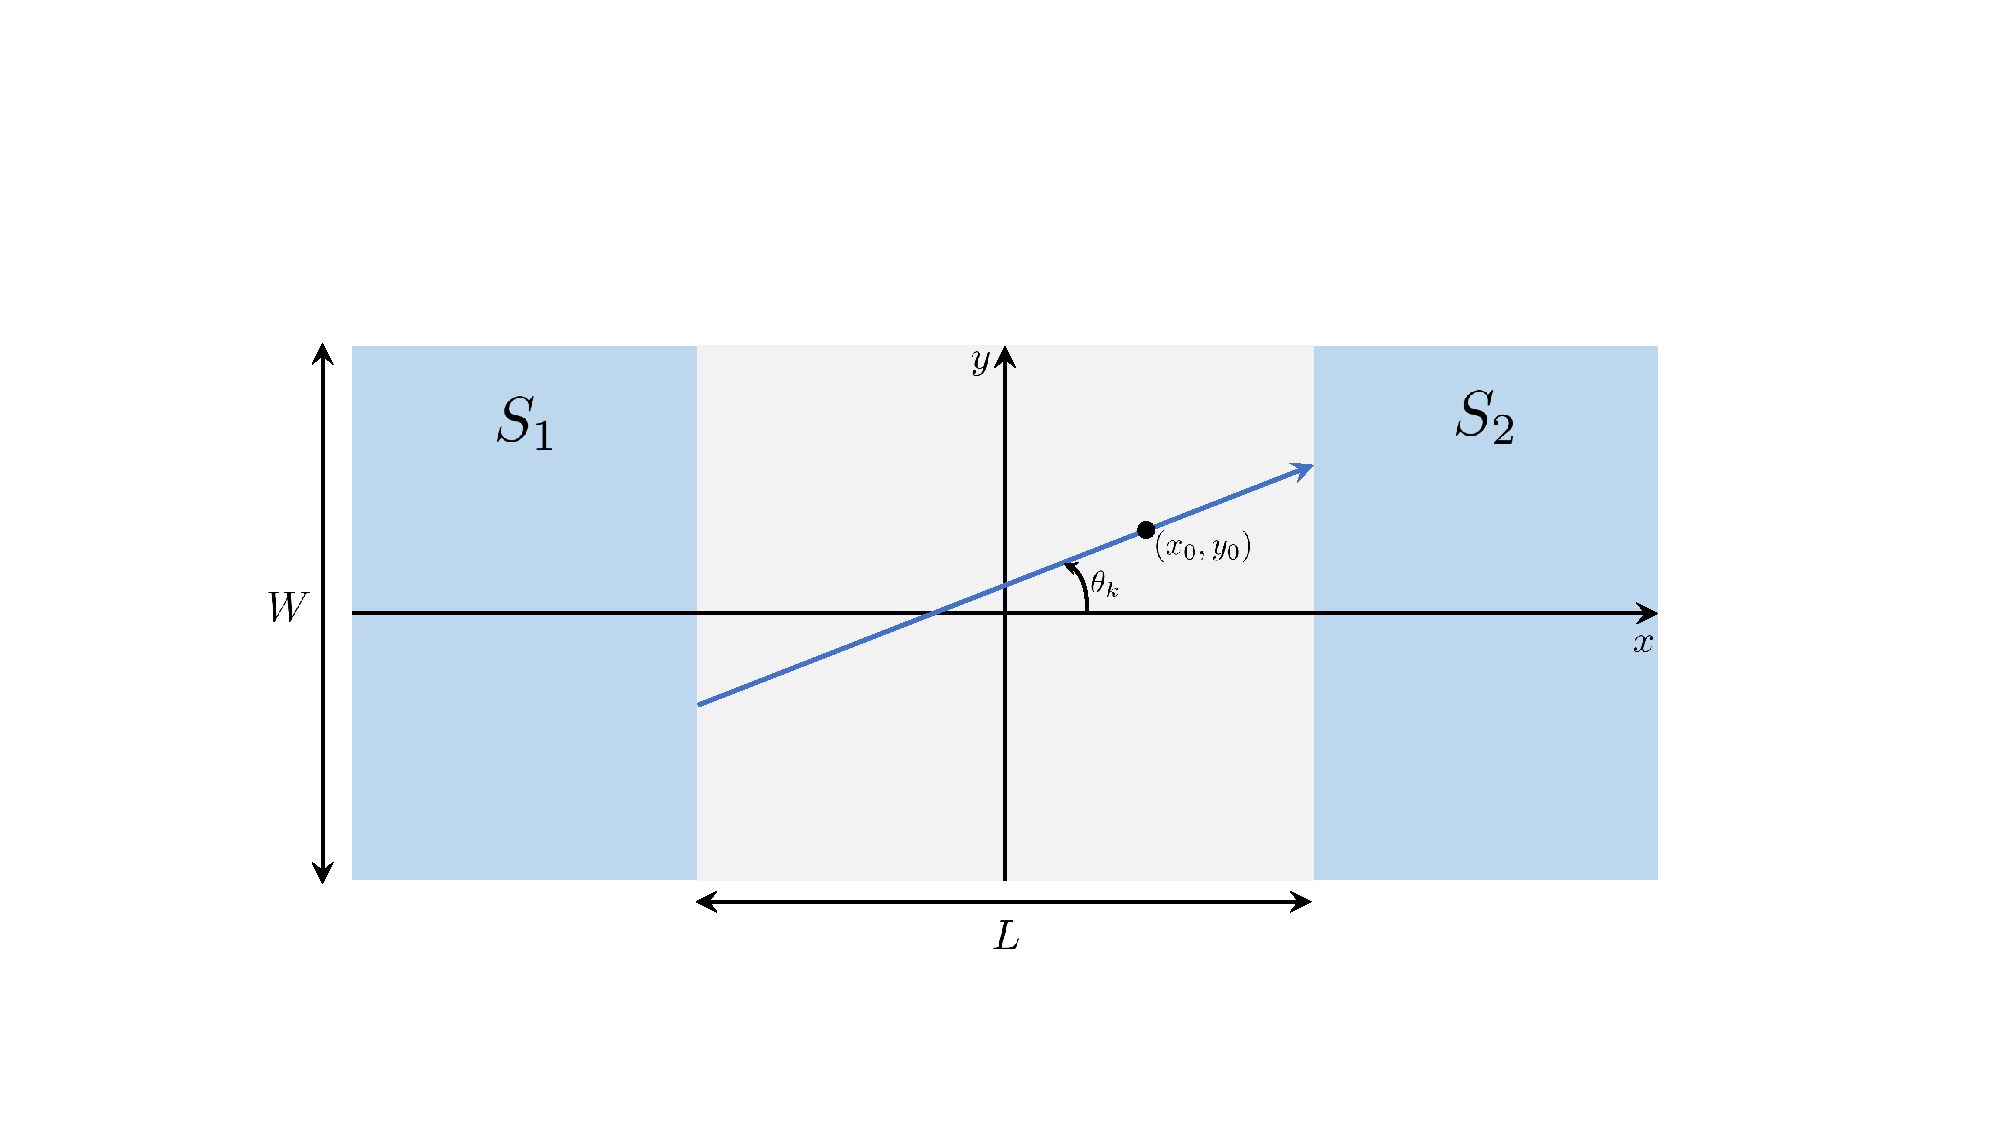
\includegraphics[width=17cm,trim = 4cm 2cm 5cm 5cm, clip=true ]{fig/Explaination}
%\subfigure[]{\includegraphics[width=3.9cm]{Dustin}\label{fig:Dustin}}
%\hfill
%\subfigure[]{\includegraphics[width=3.45cm]{Martin}\label{fig:Martin}}
\caption{blabla}
\label{fig:Explaination}
\end{figure}